\documentclass[../main.tex]{subfiles}

\begin{document}

The pipeline is triggered on push to \textit{main} branch. At first, \textit{SNAPSHOT} job is being started. Using maven, it compiles the source code, runs all the tests (both unit and integration ones), and finally, it checks the formatting based on a defined template, e.g. \textit{eclipse-codeStyle.xml}\footnote{\url{https://github.com/project-ncl/reqour/blob/akridl-thesis/eclipse-codeStyle.xml}}. In case this succeeds, built artifacts are deployed to JBoss Nexus repository\footnote{\url{https://repository.jboss.org/nexus/content/repositories/snapshots/org/jboss/pnc/reqour/}}. Some of them will be fetched and used in future stages of the pipeline.

If \textit{SNAPSHOT} job is successful, other 3 jobs are run:
\begin{itemize}
    \item \textbf{reqour-image job:} Triggers \textit{reqour-image} pipeline at GitLab using its REST API\footnote{\url{https://docs.gitlab.com/ee/ci/triggers/##trigger-a-pipeline}}.

    \item \textbf{reqour-adjuster-image job}: Same as \textit{reqour-image} job, but triggers \textit{reqour-adjuster-image} pipeline.

    \item \textbf{sonarqube job:} Runs static analysis using Sonarqube.
\end{itemize}

The above description is visualized in Figure \ref{fig:jenkins}.

\begin{figure}
  \begin{center}
    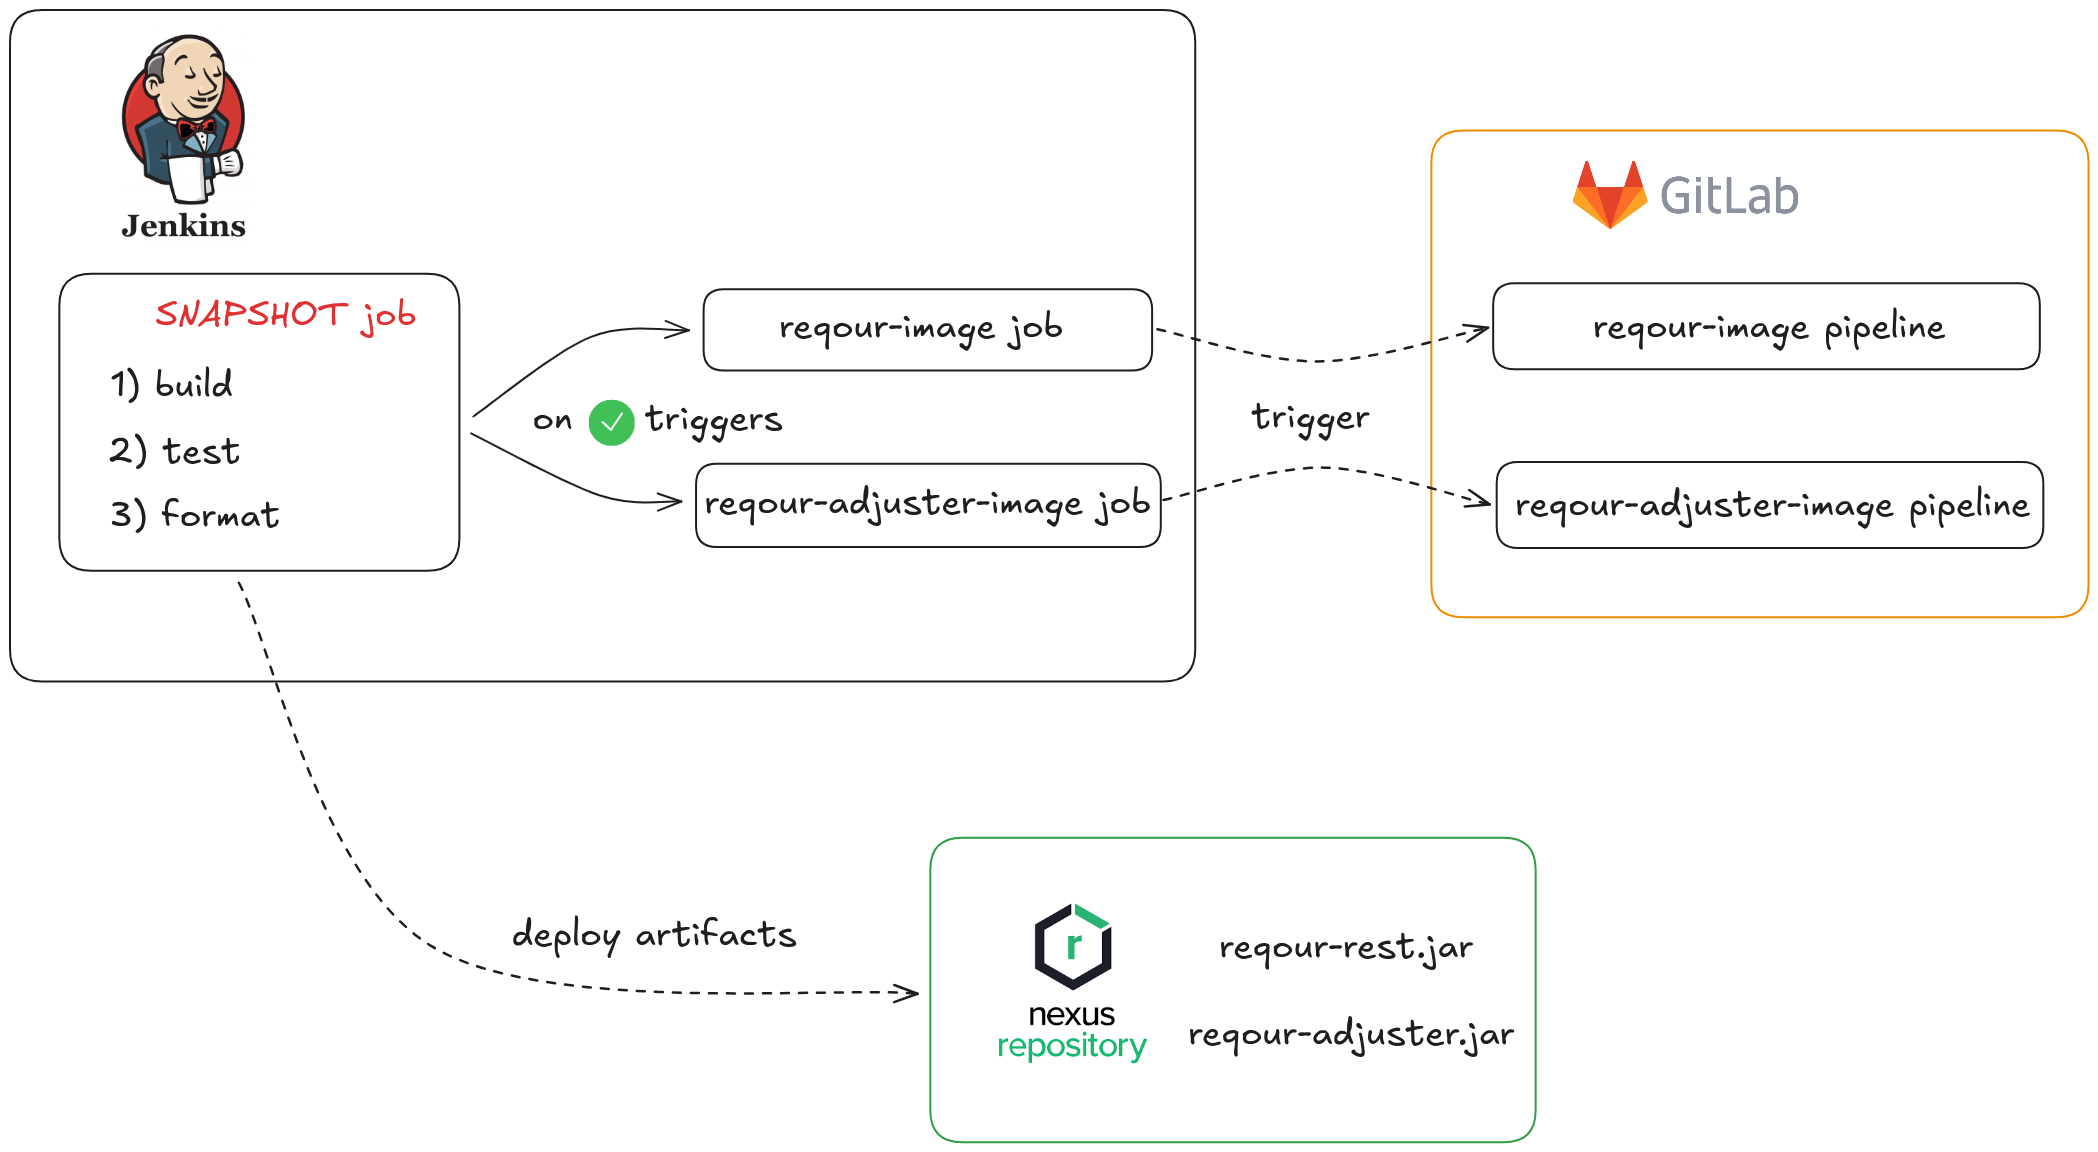
\includegraphics[width=\textwidth]{images/jenkins.png}
  \end{center}
  \caption{Jenkins part of the pipeline}
  \label{fig:jenkins}
\end{figure}

\end{document}
